\documentclass[12pt,mathserif,compress]{beamer}

\beamertemplateshadingbackground{black!5}{black!20}
\usepackage[spanish]{babel}
\usepackage{times}
\usepackage[T1]{fontenc}
\usepackage[utf8]{inputenc}
\usepackage{graphicx}
\usepackage{tikz}
\usepackage{listings}

%\usepackage{pgfpages}
%\pgfpagesuselayout{4 on 1}[a4paper,border shrink=5mm]

\renewcommand\shorthandsspanish{}
\noextrasspanish

\title{Python}
\author{Guillem Borrell i Nogueras}

\begin{document}

\lstset{language=Python,
  backgroundcolor=\color{white},
  numbers=left,
  basicstyle=\small\ttfamily,
  keywordstyle=\color{blue},
  extendedchars=true,
  inputencoding=utf8,
  showspaces=false}

\begin{frame}
\begin{center}
 
\includegraphics[width=9cm]{files/python-logo-generic.pdf}\\
 % python-logo-generic.pdf: 389x115 pixel, 72dpi, 13.72x4.06 cm, bb=0 0 389 115
\vspace{1cm}
Guillem Borrell i Nogueras\\

Físicas UCM, 18 Nov 2009
\end{center}
\end{frame}

\begin{frame}
  \frametitle{¿De qué hablará este?}
  \tableofcontents
\end{frame}
\section{¿Quién es este?}
\begin{frame}
  \frametitle{Antes de empezar}
  \begin{itemize}
  \item Guillem Borrell i Nogueras.
    \begin{itemize}
    \item  \url{http://guillemborrell.es/}
    \end{itemize}
  \item Ingeniero Aeronáutico
    \begin{itemize}
    \item Nunca me han gustado especialmente los aviones
    \end{itemize}
  \item Laboratorio de Mecánica de Fluidos Computacional
    \begin{itemize}
    \item Turbulencia en pared
    \end{itemize}
  \item Consultor de Englobe Technologies
    \begin{itemize}
    \item Supercomputación
    \end{itemize}
  \end{itemize}
\end{frame}

\begin{frame}
\frametitle{El software libre y un servidor}
\begin{itemize}
\item Empecé programando en Basic con un MSX y un monitor monocromo
  \textcolor{orange}{naranja}. Me gustaba.
\pause
\item Mis padres me compraron un PC con windows 3.11. Aprendí
  MS-DOS.
\pause
\item Windows 95 me hizo odiar el ordenador. Lo usaba para jugar al
  Civilization II.
\pause
\item En 3º un colega teleco me pasó un Red Hat 8.  Usé Octave para
  mis prácticas de Numérico II.
\end{itemize}
\end{frame}

\begin{frame} \frametitle{Entonces llegó un verano de insomnio}
\begin{center}
 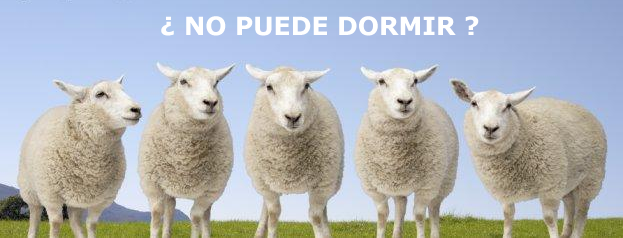
\includegraphics[width=\textwidth]{files/insomnio-ovejas.png}\\
\end{center}
\end{frame}

\begin{frame}
  \begin{center}
    Recordé lo bien que lo pasaba con el MSX de pequeño.
  \end{center}
\end{frame}

\begin{frame}
  \frametitle{Instalé un cluster casero en Gentoo Linux}
  \begin{center}
 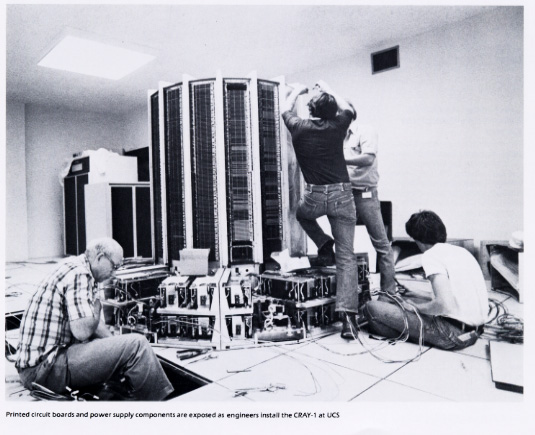
\includegraphics[width=0.8\textwidth]{files/ucs_Cray1_install.jpg}    
  \end{center}
\end{frame}

\begin{frame}
  \frametitle{Escribí un libro sobre Matlab y Octave}
  \begin{center}
  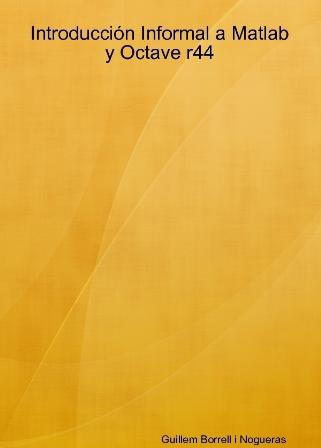
\includegraphics[height=0.6\textheight]{files/portada.jpg}    
  \end{center}
\end{frame}

\begin{frame}
  \begin{center}
    El insomnio no se fue, así que me tomé un año sabático.
  \end{center}
\end{frame}

\begin{frame}
  \frametitle{Aprendí cosas que no se enseñan en la Universidad}
Y menos aún en la Escuela de Aeronáuticos
\begin{itemize}
\item C y C++
\pause
\item Administración Linux
\pause
\item Redes
\pause
\item \textcolor{red}{\textbf{Python}}
\end{itemize}
\end{frame}

\section{¿Qué es Python?}

\begin{frame}
\frametitle{Python...}
\begin{center}
El lenguaje más versátil y consistente del mundo debe su nombre a...
\end{center}

\end{frame}

\begin{frame}
  \frametitle{Monty Python}
  \begin{center}
  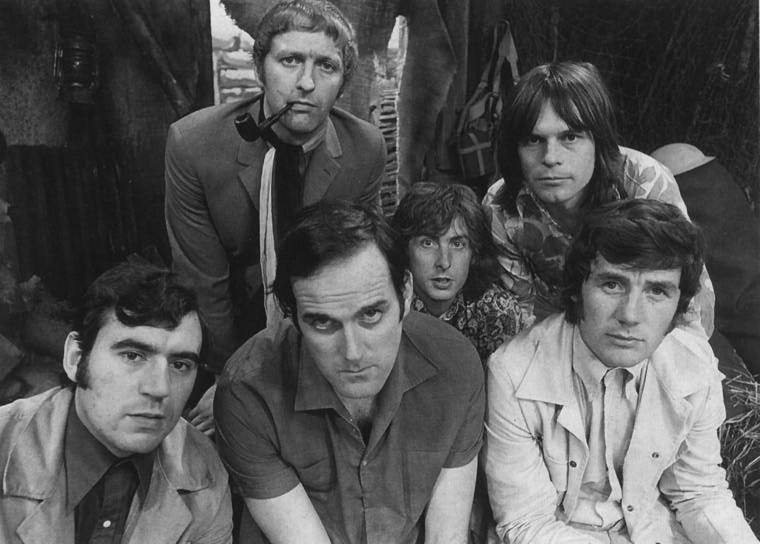
\includegraphics[width=0.8\textwidth]{files/python.jpg}    
  \end{center}
\end{frame}


\begin{frame}
  \frametitle{¿Qué es?}
Lenguaje de programación
\begin{itemize}
\item Interpretado
\item Interactivo
\item Dinámico
\item Modular
\item Orientado a objetos
\item Ampliable
\item Consistente
\end{itemize}
\end{frame}

\begin{frame}
  \begin{center}
  ¿Qué significa consistencia?    
  \end{center}
\end{frame}

\begin{frame}
  \frametitle{The Zen of Python \#13}
  \begin{center}
      \textit{Debe haber una ---mejor si es sólo una--- manera obvia de
    hacer algo}
  \end{center}
\end{frame}

\begin{frame}
  \frametitle{Interpretado}
  \begin{itemize}
  \item Python no se traduce a código máquina como C 
  \item Un compilador lo traduce a ensamblador que entiende una
    máquina virtual
  \item La máquina virtual es \emph{portable}
\pause
\item Muy portable. La \emph{misma} máquina se puede compilar en \pause
  Windows, \pause Linux, \pause Solaris, \pause AIX, \pause HP-UX,
  \pause BSD, \pause S60...
  \end{itemize}
\end{frame}

\begin{frame}
  \frametitle{Interactivo}
  \begin{center}
  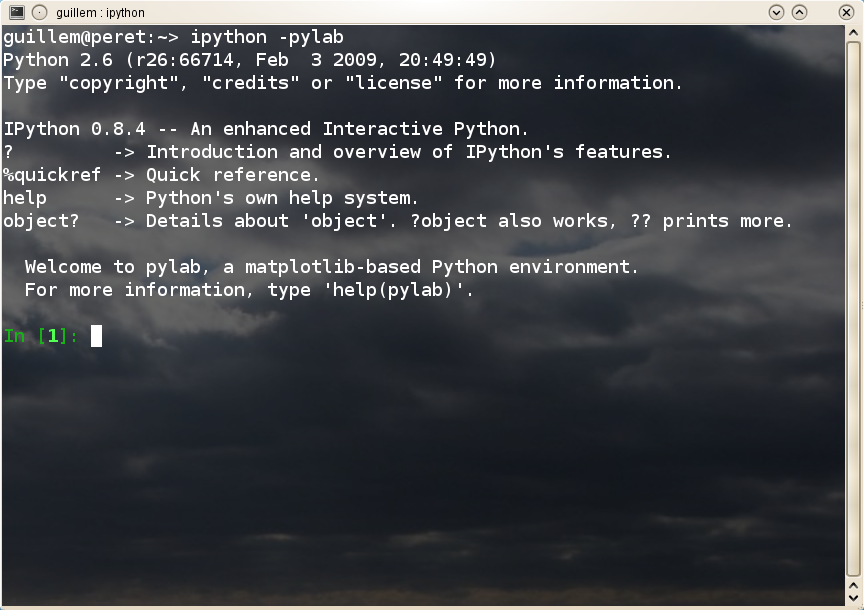
\includegraphics[width=0.8\textwidth]{files/interprete.png}    
  \end{center}
\end{frame}

\defverbatim[colored]\testcode{
\begin{lstlisting}
>>> 4.5*'hola'
TypeError: can't multiply sequence by ...
\end{lstlisting}
}
\begin{frame}
  \frametitle{Dinámico}
  \begin{itemize}
  \item No es necesario declarar variables
  \item No es necesario tipar argumentos
  \item Las variables cambian de tipo por asignación
\pause
  \item No hay conversiones de tipo implícitas
  \end{itemize}
\testcode
\end{frame}

\begin{frame}
  \frametitle{Duck Typing}
\begin{center}
\begin{tikzpicture}
\draw node[text width=0.9\textwidth, rounded corners, fill=red!20,
draw=red]
{
Si algo anda como un pato y cuaquea como un pato para mí es un pato
};
\end{tikzpicture}
\end{center}
\begin{enumerate}
\item Creamos la clase \emph{pato}
\item Creamos la clase \emph{guillem}
\pause
\item Ambos podemos decir ¡Quac!
\pause
\item Si una función llama al método \emph{cuaquea} le da igual que el
  argumento sea \emph{pato} o \emph{guillem} mientras diga ¡Quac!
\end{enumerate}
\end{frame}

\begin{frame}
  \frametitle{Modular}
  \begin{itemize}
  \item Cada archivo que contenga funciones es un módulo
  \item Cada directorio que contenga el archivo \texttt{__init__.py}
    es un módulo
  \item Tenemos la palabra clave \texttt{import}
  \item Necesaria también para la biblioteca estándar.
  \end{itemize}
\end{frame}

\defverbatim[colored]\testcode{
\begin{lstlisting}
>>> from cmath import sqrt
>>> i = sqrt(-1)
>>> i.real
0.0
>>> i.imag
1.0
\end{lstlisting}
}
\begin{frame}
  \frametitle{Orientado a Objetos}
  \begin{itemize}
  \item Todo en Python es un objeto
  \item Los módulos son objetos
  \item Casi toda la biblioteca estándar es una biblioteca de clases.
  \end{itemize}
\testcode
\end{frame}

\begin{frame}
  \frametitle{Ampliable}
\end{frame}

\section{¿Para qué uso Python?}
\begin{frame}
  \frametitle{Cálculo Numérico}
\end{frame}

\section{¿Qué hace la gente lista con Python?}

\begin{frame}
  \frametitle{Investigación sobre máquinas virtuales}
\end{frame}
\section{¿Cómo uso Python?}

\begin{frame}
  \frametitle{Un ejemplo práctico}
\end{frame}
\end{document}

